\documentclass{standalone}

\usepackage{lscape}
%Math typesetting packages
\usepackage{amsfonts, amssymb, amsmath, latexsym, amsthm,xparse, bm}
\newcommand\simiid{\stackrel{iid}{\sim}}
\newcommand\simind{\stackrel{ind}{\sim}}
\NewDocumentCommand{\qfrac}{smm}{%
  \dfrac{\IfBooleanT{#1}{\vphantom{\big|}}#2}{\mathstrut #3}%
}

\usepackage{tikz}
\usetikzlibrary{calc,arrows,positioning,shapes,shapes.gates.logic.US,trees, intersections}

\begin{document}

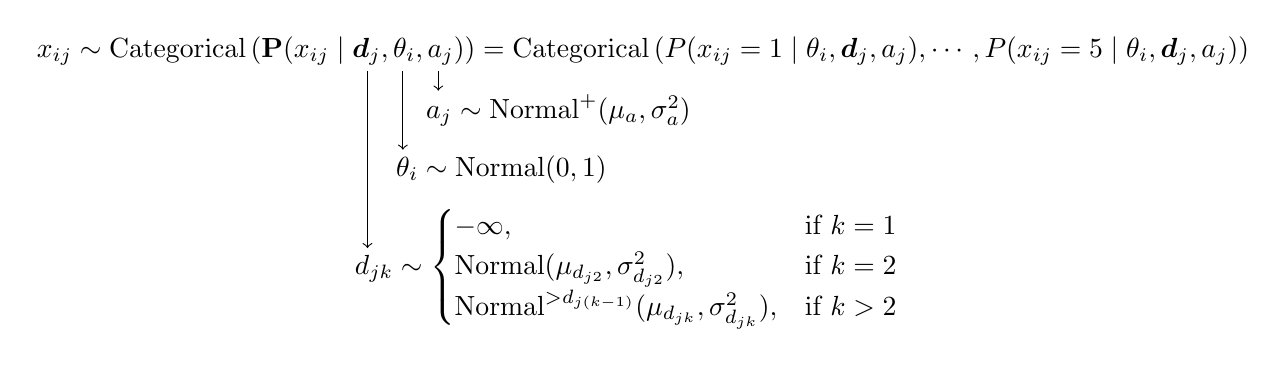
\begin{tikzpicture}
  \node at (5.2,0) {$x_{ij} \sim \mathrm{Categorical}\left(\mathbf{P}(x_{ij}\mid \bm{d}_j, \theta_i, a_j)\right)=\mathrm{Categorical}\left(P(x_{ij}=1\mid\theta_i, \bm{d}_j, a_j), \cdots, P(x_{ij}=5\mid\theta_i, \bm{d}_j, a_j)\right)$} ;
  	\draw[->] (2.6, -0.25) -- (2.6, -0.5);
  	\node at (4.125, -0.75) {$a_j\sim \mathrm{Normal}^{+}(\mu_a, \sigma^2_a)$};
  	\draw[->] (2.15,-0.25) -- (2.15,-1.25);
  	\node at (3.4, -1.5) {$\theta_i \sim \mathrm{Normal}(0,1)$};
  	\draw[->] (1.7,-0.25) -- (1.7,-2.5);
  	\node at (5, -2.75) {$d_{jk} \sim \begin{cases} -\infty, & \text{if}\ k=1\\\mathrm{Normal}(\mu_{d_{j2}}, \sigma^2_{d_{j2}}),&  \text{if}\ k=2 \\ \mathrm{Normal}^{>d_{j(k-1)}}(\mu_{d_{jk}}, \sigma^2_{d_{jk}}),& \text{if}\ k>2 \\ \end{cases}$}; 		
\end{tikzpicture}

\end{document}